%\documentstyle[epsf,twocolumn]{jarticle}       %LaTeX2e仕様
\documentclass[twocolumn]{ujarticle}     %pLaTeX2e仕様(platex.exeの場合)
%\documentclass[twocolumn]{ujarticle}     %pLaTeX2e仕様(uplatex.exeの場合)
%%%%%%%%%%%%%%%%%%%%%%%%%%%%%%%%%%%%%%%%%%%%%%%%%%%%%%%%%%%%%%
%%
%%  基本バージョン
%%
%%%%%%%%%%%%%%%%%%%%%%%%%%%%%%%%%%%%%%%%%%%%%%%%%%%%%%%%%%%%%%%%
\setlength{\topmargin}{-45pt}
%\setlength{\oddsidemargin}{0cm} 
\setlength{\oddsidemargin}{-7.5mm}
%\setlength{\evensidemargin}{0cm} 
\setlength{\textheight}{24.1cm}
%setlength{\textheight}{25cm} 
\setlength{\textwidth}{17.4cm}
%\setlength{\textwidth}{172mm} 
\setlength{\columnsep}{11mm}

\kanjiskip=.07zw plus.5pt minus.5pt


% 【節が変わるごとに (1.1)(1.2) … (2.1)(2.2) と数式番号をつけるとき】
%\makeatletter
%\renewcommand{\theequation}{%
%\thesection.\arabic{equation}} %\@addtoreset{equation}{section}
%\makeatother

%\renewcommand{\arraystretch}{0.95} 行間の設定

%%%%%%%%%%%%%%%%%%%%%%%%%%%%%%%%%%%%%%%%%%%%%%%%%%%%%%%%
\usepackage[dvipdfmx]{graphicx}   %pLaTeX2e仕様(\documentstyle ->\documentclass)\documentclass[dvipdfmx]{graphicx}
\usepackage[subrefformat=parens]{subcaption}
%%%%%%%%%%%%%%%%%%%%%%%%%%%%%%%%%%%%%%%%%%%%%%%%%%%%%%%%

\begin{document}

\twocolumn[
\noindent

\hspace{1em}
\today
\hfill
\ \ 細川 岳大

\vspace{2mm}

\hrule

\begin{center}
{\Large \bf 進捗報告}
\end{center}
\hrule
\vspace{3mm}
]

% ‚ここから 文章 Start!
\section{今週やったこと}
\begin{itemize}
	\item Embedded Residual Block Network \cite{qiu2019embedded}の実験
\end{itemize}
\section{実験}
\ Embedded Residual Block Network(:EBRN) は Block Residual Module(:BRM) が複数重なって形成される.
図\ref{fig:EBRN_model} にEBRNのモデルを示す.
\begin{figure}[ht]
	\centering
	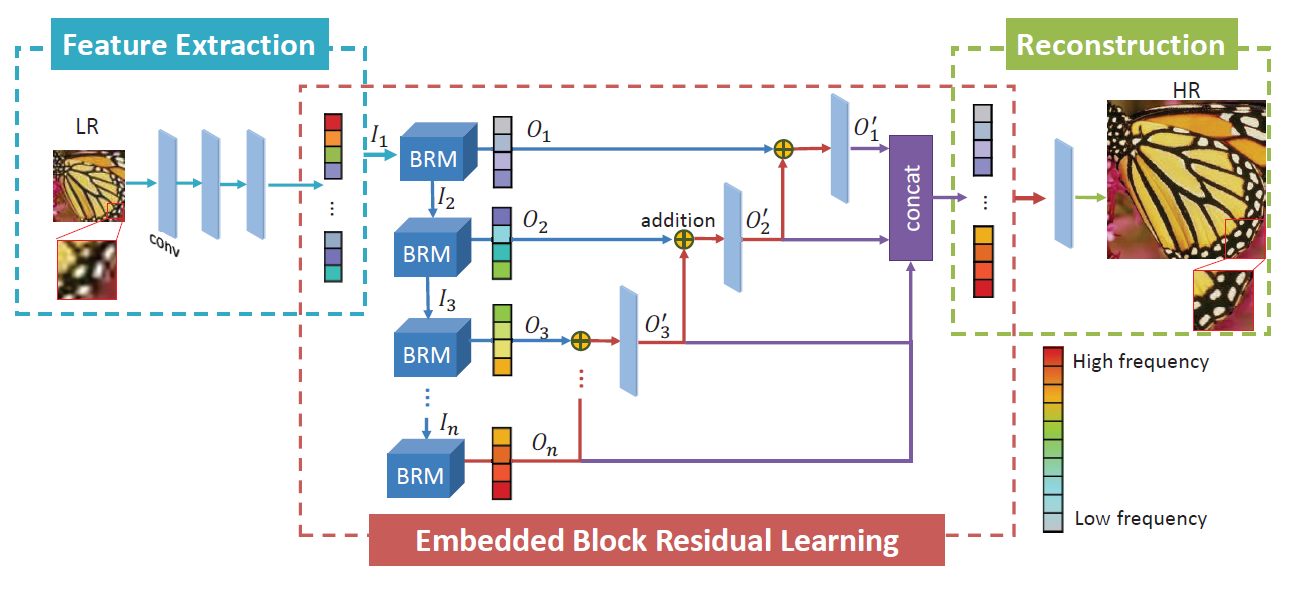
\includegraphics[]{EBRN_model.PNG}
	\caption{EBRNの概略図\label{fig:EBRN_model}}
\end{figure}
\subsection{Block Residual Module}
\ 図\ref{fig;BRM_model.PNG} にBRMの構造を示す.より下位のBRMでより画像を滑らかにする学習が行われる.
\begin{figure}[ht]
	\centering
	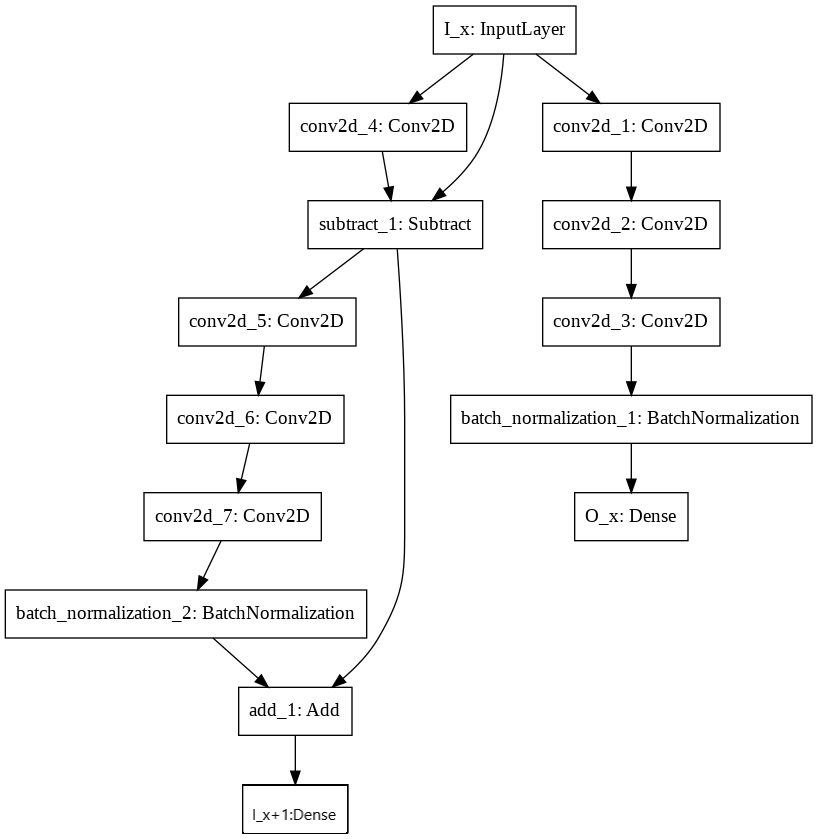
\includegraphics[]{BRM_model.PNG}
	\caption{BRMの概略図\label{fig:BRM_model}}
\end{figure}
\subsection{実験パラメータ}
表\ref{tb:param} に今回用いた実験パラメータを示す.
\begin{table}[h]
	\centering
	\caption{パラメータ\label{tb:param}
	\scalebox{0.9}{
		\begin{tabular}{|c||c|} \hline
			&ERBM\\ \hline\hline
			optimizer&Adam\\ \hline
			learning rate&0.001\\ \hline
			loss function&Mean Squared Error\\ \hline
			epoch&50\\ \hline
			batch size&16\\ \hline
		\end{tabular}
	}
\end{table}
また,初めのBRMの前に三層のCNNを積み,それぞれfilter\_sizeが256,64,24,kernel\_sizeは全て(3,3)とした.
BRM内のCNNについてのパラメータは全て等しく,filter\_sizeが24,kernel\_sizeは(3,3)とし,
BRMは12層積んだ.
最終層以外のCNNの活性化関数はPReluを用いた.
最終層のCNNはkernel\_sizeを(3,3),filter\_sizeを1,活性化関数としてmax\_valueが255のreluを用いた.
\subsection{評価手法}
\ 評価手法としてノイズの比率を表すPeak Signal-to-Noise Ratio(:PSNR)を用いた.PSNRは(1)式にて与えられる.
\begin{eqnarray}
	PSNR = 10 * \log{10}\frac{MAX^{2}_{I}}{MSE}
\end{eqnarray}
$MAX^{2}_{I}$は画素の取れる最大値であり,今回用いた画像は8bitのモノクロ画像であるので255である.
より高いほうが元画像に近いが,絶対的に信頼できる指標ではない.

\subsection{データセット}
\ データセットについて4コママンガストーリーデータセットの萌え,青年,少年の三種類のタッチ全240枚を用いる.
このうち1から8話までの192枚をtrainに,9話,10話をtestに用いる.
また,低画質画像として,情報実験2においてCAEを用いた再現画像,および四分の一に圧縮したうえでBicubic補間で元のサイズに戻したものを用いる.

\subsection{結果}
表\ref{} にPSNRの結果を示す.また図\ref{fig:train},図\ref{fig:test}に比較画像を示す.
\begin{table}[h]
	\centering
	\caption{結果\label{tb:param}
	\scalebox{0.9}{
		\begin{tabular}{|c||c|c|c|c|} \hline
			loss&val_loss&PSNR&val_PSNR\\ \hline\hline
			再現画像&1690.4333&1379.7776&15.8553&17.0312\\ \hline
			補間画像&530.6315&486.8289&20.8846&21.6216\\ \hline
		\end{tabular}
\end{table}

\begin{figure}[h]
      \begin{minipage}[t]{}
		\centering
		
\includegraphics[width=40mm]{4scale_train.png}
		\subcaption{補間画像}
      \end{minipage}  
	\begin{minipage}[t]{}
        \centering
        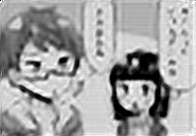
\includegraphics[width=40mm]{cae_train_decoded.png}
	\subcaption{再現画像}
      \end{minipage} \\
      \begin{minipage}[t]{}
        \centering
        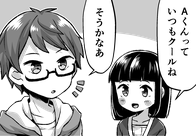
\includegraphics[width=40mm]{train_original.png}
	\subcaption{原画}
      \end{minipage}
\caption{train画像の例\label{fig:train}}
  \end{figure}

\begin{figure}[h]
      \begin{minipage}[t]{}
		\centering
		
\includegraphics[width=40mm]{4scale_test.png}
		\subcaption{補間画像}
      \end{minipage}  
	\begin{minipage}[t]{}
        \centering
        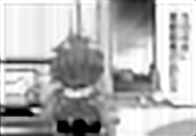
\includegraphics[width=40mm]{cae_test_decoded.png}
	\subcaption{再現画像}
      \end{minipage} \\
      \begin{minipage}[t]{}
        \centering
        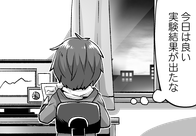
\includegraphics[width=40mm]{test_original.png}
	\subcaption{原画}
      \end{minipage}
\caption{train画像の例\label{fig:test}}
  \end{figure}

\subsection{考察}
\ CAEによって情報を落とした再現画像は超解像によって鮮明にすることは難しい.
\ Bicubic補間による画像における学習でPSNRがtestのほうがtrainよりは高いが,生成された画像についてはtrainのほうが意味ありそうなものとなったことでPSNRが絶対的な指標でないことが確認できた.またtestの生成がうまくいかない理由として,BatchSizeやfilter\_sizeが足りなかったことで過学習が起こったことが考えられる.
\section{今後の課題}
\ 

\bibliography{sa}
\bibliographystyle{unsrt}
\end{document}


